In Chapters \ref{chap:design} and \ref{chap:semantics} we defined the language structure and its semantics. We can now move onto one of the fundamental questions of this thesis (see Chapter \ref{chap:introduction}): \textit{is Casanova suitable for making games?}.

Unfortunately, fully assessing with scientific rigor the quality of a programming language is very difficult. What we will do to answer such question is the following: we will identify a series of general, orthogonal, common tasks in game development (creating a player avatar, creating an active scenario, creating a monster with an AI, etc.) and we will show how to build them in Casanova; these tasks are inspired from different sample games that we have implemented in Casanova. We believe that showing how to build these pieces of games acts as a strong indicator of the feasibility of Casanova for making games. Moreover, by comparing these snippets across different languages, we get an assessment of how Casanova fares when compared with alternate frameworks.

First we will give an overview of a small game, the \textit{Game of Life}, to see all the components of Casanova in action. Then we will show the various game development tasks.

\section{Game of Life}
The \textit{Game of Life} \cite{GAME_OF_LIFE}, depicted in Figure \ref{fig:game_of_life}, is a good starting example because it allows us to see all of the relevant features of Casanova in a very simple scenario.

\begin{figure}
\begin{center}
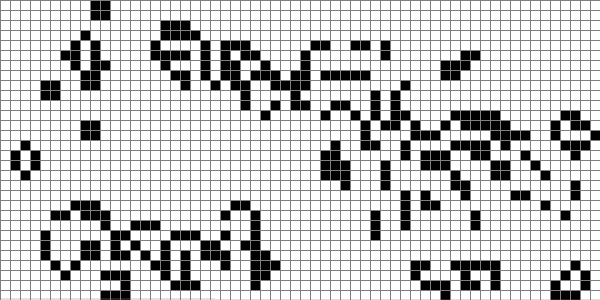
\includegraphics[width=8cm]{Pics/game_of_life.png}
\end{center}
\caption{The Game of Life}
\label{fig:game_of_life}
\end{figure}

\begin{figure}
\begin{center}
\includegraphics[width=8cm]{Pics/asteroids.png}
\end{center}
\caption{Asteroids shooter}
\label{fig:asteroids}
\end{figure}

\begin{figure}
\begin{center}
\includegraphics[width=8cm]{Pics/rpg.png}
\end{center}
\caption{RPG}
\label{fig:rpg}
\end{figure}

\begin{figure}
\begin{center}
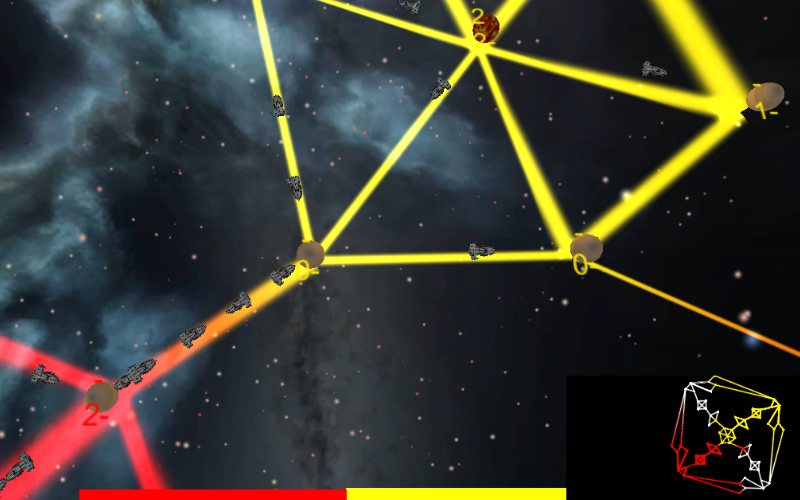
\includegraphics[width=8cm]{Pics/rts.png}
\end{center}
\caption{RTS}
\label{fig:rts}
\end{figure}

\begin{figure}
\begin{center}
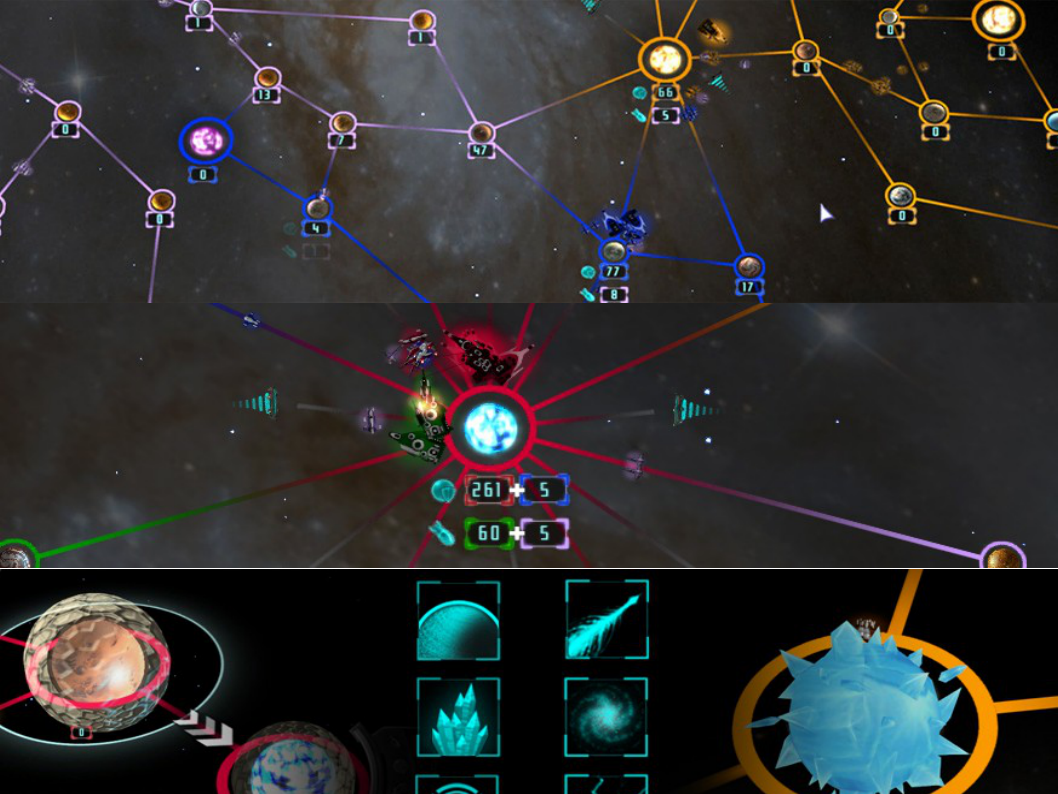
\includegraphics[width=8cm]{Pics/galaxy_wars.png}
\end{center}
\caption{Galaxy Wars}
\label{fig:galaxy_wars}
\end{figure}

The "game" is a zero-player game, meaning that its evolution is determined by its initial state, requiring no further input. One interacts with the Game of Life by creating an initial configuration and observing how it evolves.

The game is a zero-player game that takes an initial configuration of an orthogonal grid of square cells, and then evolves automatically. The player simply observes such evolution. Each cell is in one of two possible states: alive or dead. The state of a cell changes according to the state of its eight neighbors. At each iteration of the game, all cells transition in state according to the following simple rules: \textit{(i)} any live cell with fewer than two live neighbors dies; \textit{(ii)} any live cell with two or three live neighbors remains alive; \textit{(iii)} any live cell with more than three live neighbors dies; and \textit{(iv)} any dead cell with exactly three live neighbors becomes alive.

A Casanova game begins with the definition of a series of data structures, which are the world and its entities. The updates of an entity are contained in its rules, a series of methods that take the same name of the field they update at each tick; a rule is invoked automatically for each entity of the game, and it receives as input the current state of world, the current state of the entity being updated, and the time delta between the current frame and the previous frame. The result of computing a rule is stored in the game world only after all rules of all entities of the world have been computed successfully, that is, rules do not interfere with each other and can be computed in parallel. This avoids inconsistencies deriving from the state being only partially updated: the state is either at a time step or at the next, but no in-between representations are allowed. Entities may also have drawable fields such as text, sprites or 3D models; these fields are updated through rules as well, and at each tick all drawable entities are grouped into layers (layers specify blocks of drawable entities and the draw settings to use with them) which are then drawn. 

We start by defining the state of the game as a matrix of cells; the state also contains a boolean variable which will trigger the update of the cell matrix once per second. The world does not feature a sprite layer because for games that use only one sprite layer Casanova provides the developer with a predefined one that is called \texttt{default\_layer}:

\begin{lstlisting}
type World = { 
  Cells : List<List<Cell>> 
  UpdateNow : Var<bool> 
}
\end{lstlisting}

Each cell contains a value (which is 1 when the cell is alive and 0 when the cell is dead) and a list of its neighbors marked as \texttt{Ref}. The neighbors of a cell are just references to those cells, which are stored elsewhere in the game state. We inform Casanova of this fact by using \texttt{Ref}, thereby preventing Casanova from updating and drawing those cells every time they are reached from the game world. The value of the cell is updated every time an update is triggered (rather than at each tick), by summing the value of the neighbors and applying the rules mentioned above. The color of the cell sprite is updated to reflect its current value. 

\begin{lstlisting}
type Cell = { 
  NearCells : List<Ref<Cell>> 
  Value : int 
  Sprite : DrawableSprite }
  rule Value(world,self,dt) = 
    if state.UpdateNow then 
      let around = sum [for c in self.NearCells do yield c.Value] 
      match around with 
      | 3 -> 1 
      | 2 -> self.Value 
      | _ -> 0 
    else self.Value 
  rule Sprite.Color(world,self,dt) = 
    if self.Value = 0 then 
      Color.Black 
    else 
      Color.White
\end{lstlisting}

The initial state of the game creates the matrix of cells and initializes their neighbors. Each internal cell has exactly eight neighbors. The sprites layer and the cell sprite are also setup for each sprite. We omit only this listing as it is rather straightforward. The rules of the game are fired at every frame of the game that is roughly 60 times per second. Changing the entire matrix of cells this often would yield a chaotic result; for this reason we have defined the \texttt{UpdateNow} field in the game state, so that we can control when the rules are fired. The main script of the Game of Life simply waits for a second before toggling the \texttt{UpdateNow} value, and then it suspends itself until the next iteration of the update loop. When the script is resumed, it toggles \texttt{UpdateNow} again and finally it repeats. 

\begin{lstlisting}
let main world = 
  repeat co{ 
    do! wait 1.0<s> 
    world.UpdateNow := true 
    do! yield 
    world.UpdateNow := false } 
\end{lstlisting}

We could also add some basic interactivity by defining an input script which toggles updates when the user performs some input action.

\begin{lstlisting}
let input = [
    co{  
      do! wait_condition is_mouse_clicked
      do! wait_condition is_mouse_released
      return true } =>
     co{
       world.UpdateNow := true
       do! yield
       world.UpdateNow := false }
  ]
\end{lstlisting}

This way the game of life will tick at one step per second, no matter the framerate of the simulation, or when the user clicks the mouse. This is all there is to such a simple game.

\section{Making games with Casanova}
To assess the effectiveness of Casanova as a game development language we have undertaken two parallel development initiatives. The first initiative is \cite{CASANOVA_CODEPLEX}, where we have built a series of small samples that are easy to understand and manipulate; these samples are three different real-time games, chosen so as to see Casanova in action in different sub-domains of the real-time game genre, which we argue to be currently the most widespread. The second initiative is the game  \cite{GALAXY_WARS}, where we have used Casanova to build a much bigger game in order to test how well the language scales.

The small samples are an asteroid shooter game (Figure \ref{fig:asteroids}), an action/adventure game (Figure \ref{fig:rpg}), and a strategy game (Figure \ref{fig:rts}). We will not present the full samples themselves, which are available online. Instead, we will focus on a series of fundamental "development activities" that we believe to be nicely exemplified by our samples; these activities cover some of the most common and important pieces that can be customized, combined and extended into almost any game: \textit{(i)} defining a player avatar, handling his input and his shooting; \textit{(ii)} spawning obstacles randomly; \textit{(iii)} handling collisions between projectiles and obstacles; \textit{(iv)} representing the properties of a static map (cave) divided in rooms and cells; \textit{(v)} handling monsters and their AI (albeit a rudimentary one); \textit{(vi)} active entities such as bases or buildings that produce units; \textit{(vii)} selection-based input mechanisms. We show \textit{(i)}, \textit{(ii)}, and \textit{(iii)} from the asteroid shooter; \textit{(iv)} and \textit{(v)} are taken from the action/adventure game; finally, \textit{(vi)} and \textit{(vii)} are shown from the RTS game. 

By showing how to build these primitives in relative isolation from each other, we are effectively giving a library \footnote{Or rather a cookbook.} that allows to create games where a player avatar may interact with obstacles in arbitrary rooms, and where some objects are shot by the players, others simply store useful properties of the map, others move and have some AI, and others spawn units or manipulate the game world. From our experience, we note that many games can be built recombining such components. 

Since the games we present are simplified (it would be prohibitively difficult to build three large-scale games in this context) it is important to notice that these games represent just starting points that could be extended into full-blown games with more time and effort. An example of the extension process in action can be seen in \cite{GALAXY_WARS} (Figure \ref{fig:galaxy_wars}), an upcoming (commercial) strategy game that is derived from the RTS sample and that we built as an extended study of how to create non-trivial games with Casanova. Notice that the samples shown below simply are some of the most representative snippets, that is the omitted entities (for example asteroids and projectiles) are not significantly more complex than those shown in the following. 

Galaxy Wars is not the only project where Casanova has been used as a means rather than an end, even though it is the biggest. Casanova has also been used to build: \textit{(i)} two virtual city simulators that act as a testbed for AI techniques as part of a separate research effort; \textit{(ii)} an experimental AI for real-time planning; \textit{(iii)} a platform for building RTS games for both teaching and a Master Thesis; and \textit{(iv)} a serious game that teaches players cooperation in order to make a virtual organization survive. All of these examples can be accessed from the Casanova website \cite{CASANOVA_CODEPLEX}.


\section{Player avatar and shooting stuff}
The asteroid shooter game is a simple shooter game where asteroids fall from the top of the screen towards the bottom. The player aims the cannon and shoots the asteroids to prevent them from reaching the bottom of the screen. In this game we will describe how to define: \textit{(i)} the player avatar, his movement and shooting; \textit{(ii)} the spawning of obstacles such as asteroids; and \textit{(iii)} detection of collisions between asteroids and projectiles. The game world contains a list of projectiles, asteroids, the cannon, the current score, plus sprite layers for the main scene and the game UI \footnote{Compared to the Game of Life sample, here we need different sprite layers, and so we cannot rely on the default layer but instead we must declare our own.}. The game world removes asteroids and projectiles when they exit the screen or collide with each other, and it handles the current score (which is the number of destroyed asteroids). 

\begin{lstlisting}
type World = { 
  Sprites : SpriteLayer 
  UI : SpriteLayer

  StarsSprite : DrawableSprite 
  ScoreText : DrawableText

  Asteroids : Var<List<Asteroid>> 
  Projectiles : Var<List<Projectile>> 
  Cannon : Cannon 
  Score : int } 
  rule Asteroids(world,dt) = 
    [for a in state.Asteroids do 
       if a.Colliders.Length = 0 && a.Position.Y < 100.0<m> then
         yield a] 
  rule Projectiles(world,dt) = 
    [for p in state.Projectiles do 
       if p.Colliders.Length = 0 && p.Position.Y > 0.0<m> then
         yield p] 
  rule Score(world,dt) = 
    world.Score + 
      sum [for a in state.Asteroids do 
             if a.Colliders.Length > 0 then 
               yield 1]
  rule ScoreText.String(world,dt) = 
    "Current score = " + world.Score.ToString()
\end{lstlisting}  

% todo: split or expand
The player is represented by a cannon (similarly it might be represented by a moving ship) as an entity that contains a sprite, an angle, and a movement flag set from the input script that determines the variation of the angle and which is reset to 0 at every tick; the rotation of the sprite is taken from the current angle of the cannon:

\begin{lstlisting}
type Cannon = {  
  Sprite : DrawableSprite 
  Angle : float<rad> 
  Movement : Var<float> } 
  rule Angle(world,self,dt) = 
    self.Angle + self.Movement * dt
  rule Movement(world,self,dt) = 0.0
  rule Sprite.Rotation(world,self,dt) = self.Angle 
\end{lstlisting}

The input script that modifies the rotation of the cannon simply checks if the appropriate key is currently pressed, and if so the cannon movement value is set:

\begin{lstlisting}
co{ return is_key_down Keys.Left  } => co{ state.Cannon.Movement := 1.0 }; 
co{ return is_key_down Keys.Right } => co{ state.Cannon.Movement := -1.0 };
\end{lstlisting}


Similarly, projectiles are spawned whenever the space key is pressed; contrary to movement, though, after a projectile is spawned the script waits either the release of the space key or one-tenth of a second to ensure that projectiles are not shot with a frequency of one per frame as long as the user keeps pressing the space bar. 

% todo: split or expand
It is worth noticing that such a simple activity would require a timer-based event infrastructure that can be quite tedious to write in a traditional language; for example, a timer to wait after the spawning of a projectile would need to be stored, declared, and consulted manually at each tick. Instead of writing that, in Casanova we just write the following code that automatically handles the creation and management of invisible timer variables:

\begin{lstlisting}
co{ 
   do! wait_condition (is_key_down Keys.Space) 
   do! wait_condition (is_key_up Keys.Space)
         || wait 0.1<s>
   return true } =>
co{  
  state.Projectiles.Add 
    { Sprite = { Path = "projectile.jpg"; Layer = world.Sprites } 
      Position = Vector2(50.0<m>, 0.0<m>) 
      Velocity = Vector2(cos(state.CannonAngle),sin(state.CannonAngle))
      Colliders = [] } } 
\end{lstlisting}

Asteroids are generated with a simple recursive script that waits a random amount of time and then adds the asteroid to the game world before looping:

\begin{lstlisting}
  repeat co{ 
    wait (random(1.0<s>,3.0<s>)) 
    state.Asteroids.Add 
      { Sprite = { Path = "asteroid.jpg" Layer = world.Sprites }
        Position = vector2(random(0.0<m>,100.0<m>),0.0<m>) 
        Velocity = vector2(0.0<m/s>,random(5.0<m/s>,20.0<m/s>))
        Colliders = [] } } 
\end{lstlisting}

Collision detection is simple as well: both asteroids and projectiles compute the list of colliders against themselves; this list is then used in the query shown above in the definition of the game world to cull away asteroids that are hit by projectiles:

\begin{lstlisting}
type Asteroid = { 
  ...
  Colliders : List<Ref<Projectile>> } 
  ...
  rule Colliders(world,self,dt) = 
    [for x in world.Projectiles do
       if distance(self, x) < 10.0f then
         yield ref x] 
\end{lstlisting}

\section{Game map and monsters with AI}
The action/adventure game features a player-controlled character that moves between various rooms fighting monsters and drinking health-increasing potions. In the game we see how to handle: \textit{(iv)} a game world comprised of rooms and cells, where each room is divided into cells; and \textit{(v)} monsters who fight against the player with some AI. 

% todo: expand
The game state contains, among other entities (such as the player) and sprite layers (to draw the game entities and the UI) the current room the player is in. A room is defined as a series of cells and a list of monsters; monsters are removed from a room whenever they are killed when fighting against the player:

\begin{lstlisting}
type Room = { 
  Cells    : List<List<Cell>> 
  Monsters : list<Monster> } 
  rule Monsters(world,self,dt) = 
    [for m in self.Monsters do 
       if m.Health > 0 then
         yield m]
\end{lstlisting}

% todo: expand; we could instead have defined another type of cell, the portal cell, which contains ...
Each cell contains, most notably, a nullable reference to the room it leads to in case it is a portal, a list of neighboring cells, a boolean value that determines if the player is in the cell, plus a sprite for drawing it:

\begin{lstlisting}
type Cell = { 
  Position   : Vector2<m> 
  Sprite     : DrawableSprite 
  HasPlayer  : bool
  Door       : Option<Ref<Room>> 
  Neighbours : list<ref<Cell>> } 
  rule HasPlayer(world,self,dt) = 
    world.Player.Position = self 
\end{lstlisting}

% todo: expand; movement, fighting, appearance
Monsters are one the most important entities of the game. A monster contains fields to describe its position (the cell it’s currently in), its target (the cell it’s traveling to), the delta of its position between the current cell and the target cell, its sprite (for drawing it) and its current health. The monster rules update all of its fields; its health is updated when the player is in the same cell, the current cell is changed when the target cell is reached (and the target cell is set to null to stop the movement), and so on:

\begin{lstlisting}
type Monster = { 
  Position      : Var<Ref<Cell>> 
  Sprite        : DrawableSprite
  Health        : int
  Damage        : Var<int> 
  MoveTarget    : Var<Ref<Option<Cell>> 
  PositionDelta : Vector2 } 
  member Movement(world,self,dt,on_arrived,on_moving) = 
    match self.MoveTarget with 
    | Some target 
        when distance(self.Position + self.PositionDelta, 
                      target.Position) < 0.1 -> 
      on_arrived target 
    |Some target -> on_moving() 
    | None -> on_moving() 
  rule Health(world,self,dt) = 
    if self.Position.HasPlayer && world.UpdateNow then 
      self.Health - world.Player.Damage * random(1,4) 
    else self.Health 
  rule Position(world,self,dt) = 
    Movement(world,self,dt,id,
             fun () -> self.Position) 
  rule MoveTarget(world,self,dt) = 
    Movement(world,self,dt,fun () -> None,
             fun () -> self.MoveTarget)   
  rule PositionDelta(world,self,dt) = 
    Movement(world,self,dt, 
      fun () -> self.PositionDelta + 
                  dt * normalize(target.Position - 
                                 self.Position.Position), 
      fun () -> self.PositionDelta) 
  rule Sprite.Position(world,self,dt) = 
    self.Position + self.PositionDelta
\end{lstlisting}

% todo: expand, re-order
Two things in particular should be noted in the listing above. We used higher-order-functions \footnote{Higher-order-functions are those which take as some of their input parameters other functions.} to abstract away the boilerplate pattern of evaluating something when the monster is moving, and something else when the monster is still; we do so in the \texttt{Movement} method, which takes as input the \texttt{on\_arrived} and \texttt{on\_moving} functions and then invokes them as appropriate. We use the \texttt{Movement} method in the \texttt{Position}, \texttt{MoveTarget}, and \texttt{PositionDelta} rules, instead of repeating the almost identical code every time. Also, we make use of a global boolean variable, \texttt{world.UpdateNow}, which is ticked by a script and which is used as a guard to compute rules such as those for the monsters battles; this boolean is similar to the \texttt{UpdateNow} boolean that we have seen in the Game of Life. 

Monsters also have a rudimentary AI which chooses a destination cell for the monster to travel to, and which keeps doing so until the player is in the current room. This allows monsters to not weigh computationally when the player cannot interact with them, since he is in a different room. 

% todo: expand "let target_cell = ..."
\begin{lstlisting}
let monster_AI (monster : Monster) = 
  repeat co{ 
    if monster.Health > 0 then  
     if world.UpdateNow && random(0, 20) < 1 && 
        monster.MoveTarget = None then 
       let target_cell = ...
       do monster.MoveTarget := Some target_cell) } 
     || co{ wait_condition (fun () -> 
              world.CurrentRoom <> monster.Position.Room)
\end{lstlisting}

% todo: expand
Notice the use of the \texttt{(||)} operator which runs two scripts concurrently, that is until either of the scripts has completed; its use in this scenario allows us to stop the repeating script as soon as the current room changes: this disables the script for the monsters in the previous room, thereby avoiding to accumulate wasteful running scripts for rooms visited previously.

\section{Active map entities and selection-based input} 
The strategy game features a series of planets that produce ships, which can then be sent to conquer other planets. In this game we see: \textit{(vi)} active entities, such as planets, that represent complex components of the game scenario; and \textit{(vii)} complex selection-based input mechanisms based on the selection of game entities and the interaction with the selected entities.

% todo: expand
We represent the game world as a series of planets, ships, plus the currently selected planet; the game world also contains sprite layers for rendering the game entities and UI, plus a boolean that (in the same spirit of the \texttt{UpdateNow} field in the Game of Life) allows the game battles to tick at fixed time intervals rather than at each tick of the game:

\begin{lstlisting}
type World = { 
  Sprites      : SpriteLayer 
  UI           : SpriteLayer 
  Planets      : List<Planet> 
  Fleets       : Var<List<Fleet>> 
  TickBattles  : Var<bool> 
  SourcePlanet : Var<Option<Ref<Planet>>> } 
  rule Fleets(world,dt) = 
    [for f in self.Fleets do
       if f.Alive && (not(f.Arrived) || f.Fighting) then
         yield f]
\end{lstlisting}

Planets manage the battles in their orbit (to determine the owner of the planet) and ship production; in addition to their other fields, planets store the current owner, the number of allied ships stationed on the planet, and the percentage of production for the next ship; furthermore, a planet maintains a list of the fleets that are attacking or defending it:

\begin{lstlisting}
type Planet = { 
  Owner             : Player
  Armies            : Var<int<Ship>>
  FractionalArmies  : float<Ship>
  AttackingFleets   : List<Ref<Fleet>>
  ReinforcingFleets : List<Ref<Fleet>>
  ... } 
  rule Owner(world,self,dt) = 
    if self.Armies <= 0 && self.AttackingFleets.Length > 0 then
      self.AttackingFleets[0].Owner 
    else 
      self.Owner 
  rule Armies(world,self,dt) = 
    if self.Armies <= 0 then 
      sum [for a in self.AttackingFleets do
             if a.Owner = self.AtackingFleets[0].Owner then
               yield a.Armies] 
    else 
      let damages = sum[for f in self.AttackingFleets do 
                          yield random(1,3)] * state.TickBattles 
      let reinforcements = sum[for f in self.ReinforcingFleets do
                                 yield f.Armies] 
      self.Armies + int(self.FractionalArmies) - damages + reinforcements 
  rule FractionalArmies(world,self,dt) = 
    self.FractionalArmies + (dt * self.Production) - floor(self.FractionalArmies) 
  rule AttackingFleets(world,self,dt) = 
    [for f in state.Fleets do
       if f.Target = self && f.Owner <> self.Owner && f.Arrived then
         yield f] 
  rule ReinforcingFleets(world,self,dt) = 
    [for f in state.Fleets do
       if f.Target = self && f.Owner = self.Owner && f.Arrived then
         yield f]
\end{lstlisting}

% todo: expand
Input scripts manage the selection of a new planet by waiting for a left click of the mouse and then setting the \texttt{SourcePlanet} field of the game world:

\begin{lstlisting}
co{ do! wait_condition mouse_clicked_left
    do! wait_condition mouse_released_left
    let clicked = 
      [for p in world.Planets do 
         if distance(p.Position,mouse) < 10.0 && 
            p.Owner = Human then 
           yield p] 
    if clicked <> [] then
      return Some(clicked.[0])
    else 
      return None } =>
  fun p -> co{ return world.SourcePlanet := Some(p) }
\end{lstlisting}

% todo: expand
Similarly, when the user right clicks then if there is an active selection some ships are sent:

\begin{lstlisting}
co{ do! wait_condition (mouse_clicked_right && 
                        world.SourcePlanet <> None)
    do! wait_condition mouse_released_left
    let mouse = mouse_position() 
    let clicked = 
      [for p in world.Planets do
         if distance(p.Position,mouse) < 10.0 then
           yield p] 
    match clicked with
    | clicked::_ ->
      return Some(clicked.[0],world.SourcePlanet.Value) 
    | [] ->
      return None } => 
  fun (source,target) -> co{ return mk_fleet source target } 
\end{lstlisting}


\section{Recombining the samples}
The samples just shown are simple but significant snippets extracted from existing games. They represent fundamental activities in game development, since virtually all games feature at least some of these aspects; we have shown how to implement a user-controlled player that moves and shoots, we have shown how to create active obstacles with some intelligence that make the game interesting to play, and we have shown how to define static objects that are part of the scenario and that interact with the player. The samples above have indeed been recombined in the Galaxy Wars \cite{GALAXY_WARS} game, an Open Source commercial game developed in parallel with Casanova and used as a testbed for Casanova techniques. Galaxy Wars has been built as an extended study of how to create non-trivial games with Casanova. More projects, which mostly feature research simulations, have used Casanova as their framework: from virtual cities for AI research to teaching tools and even to serious games, Casanova is being put to the test extensively.

\section{Hand written optimizations}
The presented samples show no algorithmic optimizations in place, relying entirely on the runtime to provide sufficient performance. A note must be added on the fact that Casanova easily supports any algorithmic optimizations that a game developer may need to add. The least sophisticated way to add such an optimization would very simply be to use a variable to store some optimized data structure in the game world, and then using a script to update this structure in a loop. The resulting code would have the following structure:

\begin{lstlisting}
type World = {
  ...
  OptimizedStorage : Var<OptimizedStorage>
}

...

repeat
  co{ 
    do world.OptimizedStorage := update_optimized_storage world
    do! yield  
  }
\end{lstlisting}

This techniques simply replicates a traditional game loop inside Casanova itself, in order to maintain an updated data structure that stores optimized lookup tables or other similar helps to the computation. An advantage that Casanova offers at no additional cost is that if the update of the optimized data structures of the game world is expensive, then its computation may be easily split across multiple ticks, further improving the game performance:

\begin{lstlisting}
repeat
  co{
    let step1 = update_optimized_storage1 world
    do! yield
    let step2 = update_optimized_storage1 world step2
    do! yield
    ...
    do world.OptimizedStorage := update_optimized_storageN world stepN
    do! yield  
  }
\end{lstlisting}

Of course, rules may also be used to implement such a system without scripts and mutability. A significant difference between using rules rather than scripts is that for the results of rules to propagate to other rules then it takes multiple ticks, and so rules force the developer to implement the second snippet of the two shown above. If the optimized data structure must be computed entirely in one frame, and must be updated at every frame, then scripts are the most effective solution.
